% TikZ 复刻。原图：assets/half-adjust.png
% 回退：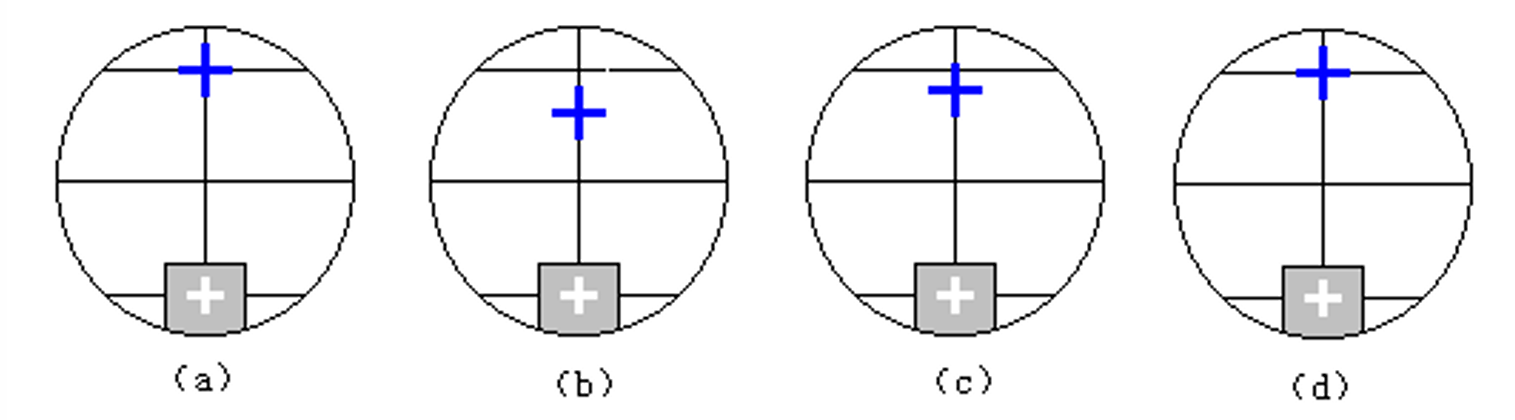
\includegraphics[width=\linewidth]{assets/half-adjust.png}
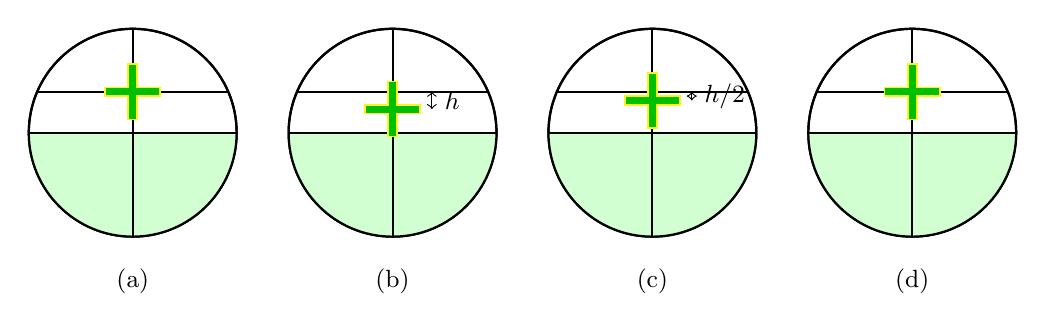
\begin{tikzpicture}[font=\small]
  \def\R{1.32}
  \foreach \xshift/\gy/\lab/\shownote/\notetext in {
      0/0.52/{(a)}/0/{},
      3.3/0.30/{(b)}/1/{$h$},
      6.6/0.41/{(c)}/1/{$h/2$},
      9.9/0.52/{(d)}/0/{}
    } {
    \begin{scope}[shift={(\xshift,0)}]
      \draw[thick] (0,0) circle (\R);
      \begin{scope}
        \clip (0,0) circle (\R);
        \fill[green!18] (-\R-0.1,-\R-0.1) rectangle (\R+0.1,0);
        \draw[line width=0.7pt] (0,-\R) -- (0,\R);
        \draw[line width=0.7pt] (-\R,0) -- (\R,0);
        \draw[line width=0.7pt] (-\R,0.52) -- (\R,0.52);
        \draw[line width=3.8pt, yellow!90] (-0.36,\gy) -- (0.36,\gy);
        \draw[line width=3.8pt, yellow!90] (0,\gy-0.36) -- (0,\gy+0.36);
        \draw[line width=2.5pt, green!75!black] (-0.34,\gy) -- (0.34,\gy);
        \draw[line width=2.5pt, green!75!black] (0,\gy-0.34) -- (0,\gy+0.34);
      \end{scope}
      \draw[thick] (0,0) circle (\R);
      \ifnum\shownote=1
        \draw[<->] (0.50,0.52) -- (0.50,\gy);
        \node[right] at (0.54,{0.5*(0.52+\gy)}) {\notetext};
      \fi
      \node[below] at (0,-\R-0.28) {\lab};
    \end{scope}
  }
\end{tikzpicture}
